% ### Erste Seite der Augenverbindungen ###
\centering
\section*{\myul{Augenverbindungen}}

% Klebefläche für das erste Register:
\begin{tikzpicture}[remember picture, overlay, x=1mm, y=-1mm]
    \begin{scope}[shift={(current page.north west)}]
        \draw (206,102) -- (202,102) -- (202,80) -- (206,80);
        \node[rotate=90, anchor=center] at (204,91) {Augen};
    \end{scope}
\end{tikzpicture}

\begin{tikzpicture}[remember picture, overlay]

% --- ERSTE REIHE: Am Seitenursprung anfangen
\setlength{\rowheight}{69mm}

    % X2) Eigene Zeile für die Überschrift
    \Tile{X1}{([xshift=10mm, yshift=-16mm]current page.north west)}{190mm}{8mm}
    {
        \titlebf{Augendimensionierung nach Roloff / Matek}
    }{0}{0}{0}{0}

    % A1) Erste Kachel unten anbauen
    \setlength{\cellwidth}{56mm}
    \Tile{A1}{(X1.south west)}{\cellwidth}{\rowheight}
    {
        \vspace{-\TileSep}
        \titlerm{Dicke des Mittleren Auges $t_\text{S}$} \\ \vspace{-2.5mm}
        \begin{equation*}
            t_\text{S} \stackrel{!}{\geq} \text{0,7}\,\sqrt{\frac{F_\text{B}~S_\text{M}}{R_\text{e}}}
        \end{equation*}
        \titlerm{Lochdurchmesser $d_\text{L}$} \\ \vspace{-3.5mm}
        \begin{equation*}
            d_\text{L} \stackrel{!}{\geq} \text{2,5}~t_\text{S}
        \end{equation*}
        \vspace{-4mm}
        {\scriptsize
        \begin{align*}
            t_\text{s} = &\text{ Dicke der Stange}                \\
            F_\text{B} = &\text{ Bemessungslast}                  \\
            S_\text{M} = &\text{ Teilsicherheitsbeiwert}          \\[-0.5ex]
                         &(\text{Allg.: }S_\text{M} = \text{1,1}) \\
            R_\text{e} = &\text{ Streckgrenze (Augenwerkstoff)}   \\
            R_\text{M} = &\text{ Zugfestigkeit (Augenwerkstoff)}  \\
            d_\text{L} = &\text{ Lochdurchmesser}
        \end{align*}
        }
    }{0}{1}{1}{0}

    % B1) Zweite Kachel rechts anbauen
    \setlength{\cellwidth}{55mm}
    \Tile{B1}{(A1.north east)}{\cellwidth}{\rowheight}
    {
        \vspace{-\TileSep}
        \titlerm{Festigkeitsbedingung} \\ \vspace{-1.5mm}
        \begin{equation*}
            \frac{K_\text{A}~F_\text{B}}{2~c~t}\left(1+\frac{3}{2}\left(\frac{d_\text{L}}{c}+1\right)\right)\stackrel{!}{\leq} \sigma_\text{zul}
        \end{equation*}
        \\ \vspace{0.8mm}
        \titlerm{Zulässige Spannung $\sigma_\text{zul}$} \\ \vspace{1mm}
        \resizebox{\cellwidth-2\TileSep}{!}{
        \begin{tabular}{c|c|c}
            \xrowht[()]{1.8mm}$\sigma_\text{zul}$ & Stahl            & GJL (GG)         \\ \hline
            \xrowht[()]{1.8mm}Stat. Belastung     & 0,5 $R_\text{e}$ & 0,5 $R_\text{m}$ \\ \hline
            \xrowht[()]{1.8mm}Dyn. Belastung      & 0,2 $R_\text{e}$ & 0,2 $R_\text{m}$
        \end{tabular}
        }\vspace{-1mm}
        {\scriptsize
        \begin{align*}
            K_\text{A}        &= \text{Anwendungsfaktor}    \\
            F_\text{B}        &= \text{Bemessungslast}      \\
            c                 &= \text{Wangenbreite (Auge)} \\
            t                 &=
            \begin{cases}
                \text{Stange: } & t_\text{S}   \\
                \text{Gabel: }  & 2~t_\text{G}
            \end{cases} \\
            d_\text{L}        &= \text{Lochdurchmesser}     \\
            \sigma_\text{zul} &= \text{Zulässige Spannung}
        \end{align*}
        }
    }{0}{1}{1}{0}
    
    % C1) Dritte Kachel rechts anbauen
    \setlength{\cellwidth}{79mm}
    \Tile{C1}{(B1.north east)}{\cellwidth}{\rowheight}
    {
        \vspace{-\TileSep}
        \begin{minipage}{0.5\cellwidth-\TileSep}
            \centering
            \titlerm{Scheitelhöhe $s$}\\ \vspace{-1.5mm}
            \begin{equation*}
                a \stackrel{!}{\geq}\frac{F_\text{B}~S_\text{M}}{2~t_\text{S}~R_\text{e}} + \frac{d_\text{L}}{3}
            \end{equation*}
            \titlerm{Wangenbreite $c$}\\ \vspace{-1.5mm}
            \begin{equation*}
                c \stackrel{!}{\geq}\frac{F_\text{B}~S_\text{M}}{2~t_\text{S}~R_\text{e}} + \frac{d_\text{L}}{3}
            \end{equation*}
            \vspace{8mm}
        \end{minipage}%
        \begin{minipage}{0.5\cellwidth-\TileSep}
            \centering
            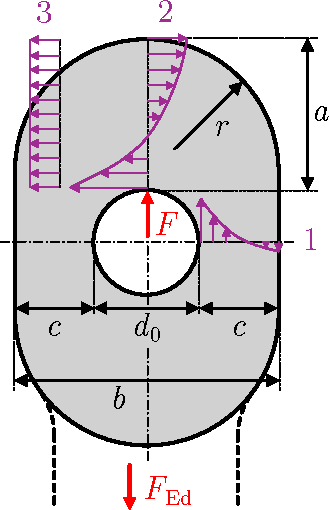
\includegraphics[width=0.8\textwidth]{images/augen-spannungen-maße.pdf}
        \end{minipage}%
        \vspace{-10mm}
        {\scriptsize
        \begin{align*}
            a          &= \text{Scheitelhöhe}                                                    \\
            F_\text{B} &= \text{Bemessungslast}                                                  \\
            t_\text{S} &= \text{Dicke der Stange}                                                \\
            R_\text{e} &= \text{Streckgrenze}                                                    \\
            S_\text{M} &= \text{Teilsicherheitsbeiwert } (\text{Allg.: }S_\text{M} = \text{1,1}) \\
            d_\text{L} &= \text{Lochdurchmesser}                                                 \\
            c          &= \text{Wangenbreite}
        \end{align*}
        }
    }{0}{0}{1}{0}

% --- ZWEITE REIHE: Am Seitenursprung anfangen
\setlength{\rowheight}{50mm}

    % X2) Eigene Zeile für die Überschrift
    \Tile{X2}{(A1.south west)}{190mm}{8mm}
    {
        \titlebf{Augen- \& Bolzendimensionierung nach Handbuch Strukturberechnung (HSB)}
    }{0}{0}{0}{0}

    % A2) Erste Kachel unten anbauen
    \setlength{\cellwidth}{42mm}
    \Tile{A2}{(X2.south west)}{\cellwidth}{\rowheight}
    {
        \vspace{-\TileSep}
        \titlerm{Lastrichtung}\\ \vspace{2mm}
        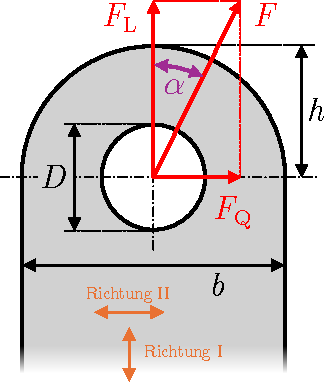
\includegraphics[width=\cellwidth-4\TileSep]{images/augen-lastrichtung.pdf}
    }{0}{1}{1}{0}

    % B2) Zweite Kachel rechts anbauen
    \setlength{\cellwidth}{70mm}
    \Tile{B2}{(A2.north east)}{\cellwidth}{\rowheight}
    {
        \vspace{-\TileSep}
        \titlerm{Fertigungsrichtung}\\ \vspace{4mm}
        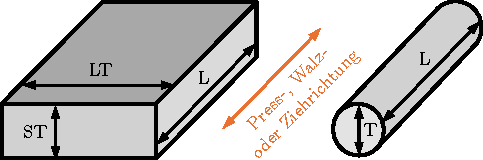
\includegraphics[width=\cellwidth-4\TileSep]{images/augen-fertigungsrichtung.pdf}\\ \vspace{4mm}
        \begin{tabular}{rlr}
             &  & Gewünscht \\
            Richtung I: & Längsrichtung & L \\
            Richtung II: & Querrichtung & LT, ST, T
        \end{tabular}
    }{0}{1}{1}{0}

    % C2) Dritte Kachel rechts anbauen
    \setlength{\cellwidth}{78mm}
    \Tile{C2}{(B2.north east)}{\cellwidth}{\rowheight}
    {
        \vspace{-\TileSep}
        \titlerm{Belastung in Längsrichtung (Richtung I)}\\ \vspace{1mm}
        \begin{equation*}
            F_\text{V} = \min\!
            \begin{cases}
                F_\text{w,V} \\
                F_\text{s,V} \\
                \text{1,5}~F_\text{FL,V}
            \end{cases}
        \end{equation*}
        {\scriptsize
        \begin{align*}
            F_\text{V}    &= \text{Versagenslast}                          \\
            F_\text{w,V}  &= \text{Versagenslast (Wangenbruch)}            \\
            F_\text{s,V}  &= \text{Versagenslast (Ausscheren im Scheitel)} \\
            F_\text{FL,V} &= \text{Versagenslast (Fließbelatung)}
        \end{align*}
        }
    }{0}{0}{1}{0}

\end{tikzpicture}